%-------------------------------------------------------------------------------
%-------------------------------------------------------------------------------
\section{Network analysis: looking for a structure}
%-------------------------------------------------------------------------------
%-------------------------------------------------------------------------------

%------------------------------------------------------------------------------
\frame{ \frametitle{Observed network}

  \begin{tabular}{ccc}
    \hspace{-.04\textwidth}
    \begin{tabular}{p{.35\textwidth}}
      \paragraph{Network} \\
      \includegraphics[width=.3\textwidth]{\fignet/SBM-Network}
    \end{tabular}
    & 
    \hspace{-.1\textwidth}
    \begin{tabular}{p{.35\textwidth}}
      \paragraph{Adjacency matrix} \\
      \includegraphics[width=.3\textwidth]{\fignet/SBM-Adjacency}
    \end{tabular}
    &
    \hspace{-.1\textwidth}
    \begin{tabular}{p{.35\textwidth}}
      \paragraph{That is}
      \begin{itemize}
        \item $n$ nodes (genes, proteins, species, \dots : $1 \leq i, j \leq n$) \\~
        \item $Y_{ij} = $ interaction between nodes $i$ and $j$
      \end{itemize}
    \end{tabular}
  \end{tabular}
  
  \bigskip \pause  
  $$
  \begin{tabular}{p{.35\textwidth}p{.35\textwidth}}
    \paragraph{Type of network:} & \paragraph{Type of edge:} \pause \\ %~ \\ 
    directed / undirected & $Y_{ij} = Y_{ji}$ or not \pause \\ %~ \\
    binary / valued ('weighted') & $Y_{ij} \in \{0, 1\}$ or $\Rbb$ \pause \\ %~ \\
    multivariate ('multiplex') & $Y_{ij} \in \{0, 1\}^d$ or $\Rbb^d$ \\ 
    & or $\{0, 1\} \times \{a, b, c, d\} \times \Nbb \times \Rbb$
  \end{tabular}     
  $$

}

%------------------------------------------------------------------------------
\frame{ \frametitle{Statistical model}

  \paragraph{Observed data.} The observed adjacency matrix 
  $$
  y = [y_{ij}]_{1 \leq i, j, \leq n}
  $$
  is a realisation of a {\sl random graph} (or random matrix)
  $$
  Y = [Y_{ij}]_{1 \leq i, j, \leq n}
  $$
  
  \bigskip \bigskip \pause
  \paragraph{Random graph model=} joint distribution of the $\approx n^2$ random values $Y_{ij}$ : 
  $$
  Y \sim p
  $$
  that is
  $$
  p(y) = \Pr\{Y_{11} = y_{11}, \dots Y_{ij} = y_{ij}, \dots Y_{nn} = y_{nn}\}
  $$

}

%==================================================================
\frame{ \frametitle{A simple random graph}

  \paragraph{Erd\"os-R\'enyi:}
  %\footnote{Alternate version $\Gcal(n, m)$, $m =$ fixed number of edges}:
  \begin{itemize}
   \item $n$ nodes (= genes, \dots) 
   \item undirected binary edges (= interactions) : $Y_{ij} = Y_{ji}  \in \{0, 1\}$
   \item all pairs of nodes are connected (= interact) independently 
   \item with same probability $\pi$
  \end{itemize}
  $$
  \{Y_{ij}\} \text{ iid } \sim \Bcal(\pi)
  $$
  
  \bigskip \bigskip \pause
  \paragraph{Properties.}
  \begin{itemize}
   \item Graph density $= \pi$ \\ ~
   \item Degree (= number of neighbors) of a node $\sim \Bcal(n-1, \pi) \approx \Pcal(n \pi)$ \\ ~
%    \ra Homegeneous degree distribution
   \item Clustering coefficient $c = P\{j \sim k \mid i \sim j, i \sim k\} = \pi$ %\\
   \qquad (no 'assortativity')
  \end{itemize}
}

%==================================================================
\frame{ \frametitle{Network analysis}

  \paragraph{Erd\"os-R\'enyi random graph.}
  \begin{itemize}
   \item Very well known and understood
   \item Does not fit most networks: all genes play exactly the same role
  \end{itemize}
  \ra Need for more complex models

  \bigskip \bigskip \pause
  \paragraph{Always the same:} What are we looking for ?
  
  \bigskip \pause
  \paragraph{Network topology (organization).}
  \begin{itemize}
  \item Node scale (degree distribution)
  \item Global scale (density, connected classes, \dots)
  \item Intermediate (e.g. node clustering: see next)
  \end{itemize}

  \bigskip \pause
  \paragraph{Network 'behavior':} e.g. is the network stable
  \begin{itemize}
  \item Relies on an implicit dynamic model
  \end{itemize}
  \ra Do we have the data to fit it?
}

%==================================================================
\frame{ \frametitle{Stochastic blockmodel}

  \bigskip
  \paragraph{Mixture model \refer{HoL79,NoS01}.} Undirected, binary version : 
  \begin{itemize}
    \item There exists $K$ groups of nodes \\~
    \item Each node $i$ belongs to one {\sl unobserved} class $Z_i$ \\~ 
    \item The probability for nodes $i$ and $j$ to be connected only depends on their respective groups :
    $$
    \Pr\{Y_{ij} \mid i \in k, j \in \ell\} = \gamma_{k\ell}
    $$
  \end{itemize}
  
  \bigskip \bigskip \pause
  \paragraph{Many avatars.} 
  \begin{itemize}
    \item Bipartite networks \refer{GoN05}, valued networks \refer{MRV10}, temporal networks \refer{MaM17}, multipartite (more than two types of nodes) \refer{BBD19}, \dots
  \end{itemize}

  \bigskip \bigskip \pause
  \paragraph{Statistical inference.} 
  Not completely straightforward because the nodes' membership $Z_i$ are not observed. 
  
  \medskip
  \ra Resort to a variational approximation of the likelihood (likewise PLN)

}

%==================================================================
\frame{ \frametitle{{\sl E. coli} operon network}

  \begin{tabular}{cc}
    \hspace{-.04\textwidth}
    \begin{tabular}{p{.5\textwidth}}
      \paragraph{Directed network.} 
      \begin{itemize}
       \item $n = 328$ operons, 
       \item 456 directed interactions :
        $$
        Y_{ij} = 1 \text{ iff $i$ 'regulates' $j$}
        $$
      \end{itemize}

      \bigskip \pause
      $$
      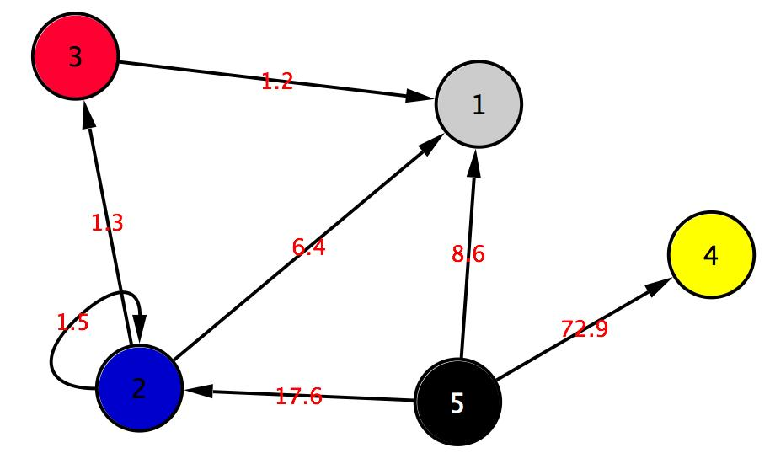
\includegraphics[width=.4\textwidth]{\fignet/VEMmetagraphe.png}
      $$
      
      \bigskip
      \paragraph{Choosing $K$:} penalized 'likelihood'
    \end{tabular}
    & 
    \begin{tabular}{p{.5\textwidth}}
      \includegraphics[width=.4\textwidth]{\fignet/im_EcoliVEM_2}
    \end{tabular}
  \end{tabular}
  
}

%==================================================================
\frame{ \frametitle{Accounting for covariates}

  \paragraph{Same story as network inference:} accounting for available information on nodes ($x_i$) or pairs ($x_{ij}$) may avoid to re-discover the wheel
  
  \bigskip \bigskip \pause
  \paragraph{Including covariates} is often easy (at least formally) adding a regression term:
  $$
  \text{logit}(\Pr\{Y_{ij} = 1 \mid Z_i=k, Z_j=\ell\}) = \alpha_{k\ell} + x_{ij}^\intercal \beta
  $$
  (where $\text{logit}(p) = \log(p/(1-p))$)
  
  \bigskip \pause
  \begin{itemize}
   \item Aims at analysing the structure of the network, that is {\sl not explained} by the covariates ('residual' structure)
%    \item The edges are not exchangeable anymore
   \item Easier to account for edge covariates ($x_{ij}$), than node covariates ($x_i$)
  \end{itemize}
  
  \bigskip \bigskip \pause
  \paragraph{Next: Poisson stochastic blockmodel with covariates:} \refer{MRV10}
  $$
  (Y_{ij} \mid Z_i=k, Z_j=\ell) \sim \Pcal(\exp(\alpha_{k\ell} + x_{ij}^\intercal \beta))
  $$

}

%====================================================================
\frame{ \frametitle{Ecological network (1/2)}

  \begin{tabular}{cc}
    \hspace{-.04\textwidth}
    \begin{tabular}{p{.4\textwidth}}
      \paragraph{Data:} 
      \begin{itemize}
       \item $n = 51$ tree species,
       \item $X_{ij}=$ number of fungal parasites shared by species $i$ and $j$ (\refer{VPD08}).
      \end{itemize}

      \bigskip \bigskip \pause
      \paragraph{Model:}
      $$
      Y_{ij} \sim \Pcal(\lambda_{k\ell}),
      $$
      $\lambda_{k\ell} =$ mean number of common parasites.

      \bigskip \bigskip 
      \paragraph{Results:} ICL selects $K=7$ groups
      that are \emphase{partly related with phylums}. \pause
    \end{tabular}
    & 
    \hspace{-.05\textwidth}
    \begin{tabular}{c}
      {\tiny
        \begin{tabular}{c|ccccccc}
          $\widehat{\lambda}_{q\ell}$ & T1 & T2 & T3 & T4 & T5 & T6 &
          T7 \\ 
          \hline
          T1 & 14.46 & 4.19 & 5.99 & 7.67 & 2.44 & 0.13 & 1.43 \\
          T2 &  & 14.13 & 0.68 & 2.79 & 4.84 & 0.53 & 1.54 \\
          T3 &  &  & 3.19 & 4.10 & 0.66 & 0.02 & 0.69 \\
          T4 &  &  &  & 7.42 & 2.57 & 0.04 & 1.05 \\
          T5 &  &  &  &  & 3.64 & 0.23 & 0.83 \\
          T6 &  &  &  &  &  & 0.04 & 0.06 \\
          T7 &  &  &  &  &  &  & 0.27 \\
          \hline \hline
          $\widehat{\alpha}_q$ & 7.8 & 7.8 & 13.7 & 13.7 & 15.7 & 19.6 &
          21.6  
        \end{tabular}
        }\\ \pause
        
        \bigskip
        $$
        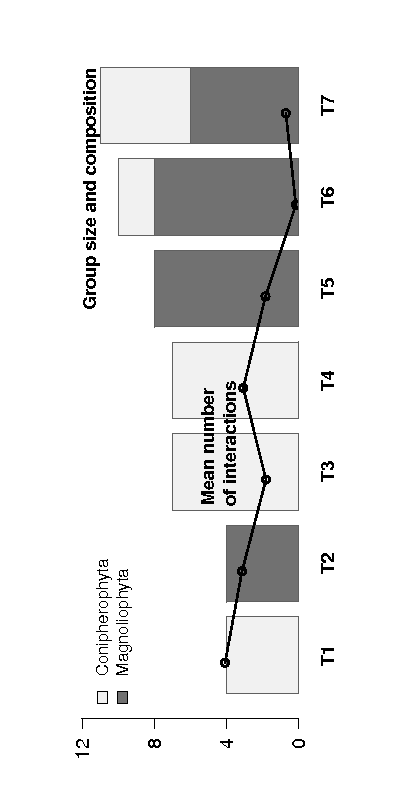
\includegraphics[width=.5\textwidth, trim=150 150 150 150, clip=]{\fignet/MRV10_AoAS_Q7_group}
        $$
    \end{tabular}
  \end{tabular}
  }

%====================================================================
\frame{ \frametitle{Ecological network (2/2)}

  \begin{tabular}{cc}
    \hspace{-.04\textwidth}
    \begin{tabular}{p{.4\textwidth}}
      \paragraph{Accounting for phylogeny:} 
      \begin{itemize}
       \item $x_{ij}=$ taxonimic distance between species $i$ and $j$.
      \end{itemize}

      \bigskip \bigskip \pause
      \paragraph{Model:}
      $$
      X_{ij} \sim \Pcal(\exp(\alpha_{k\ell} + x_{ij}^\intercal \beta)),
      $$
      \ra $\widehat{\beta} = -0.317$ (makes sense !)

      \bigskip \bigskip 
      \paragraph{Results:} ICL selects $K=4$ groups
      that are \emphase{not related with phylums}. \pause
    \end{tabular}
    & 
    \hspace{-.05\textwidth}
    \begin{tabular}{c}
      {\tiny
        \begin{tabular}{c|cccc}
          $\widehat{\lambda}_{q\ell}$ & T'1 & T'2 & T'3 & T'4 \\ 
          \hline
          T'1 & 0.75 & 2.46 & 0.40 & 3.77 \\
          T'2 &  & 4.30 & 0.52 & 8.77 \\ 
          T'3 &  &  & 0.080 & 1.05 \\ 
          T'4 &  &  &  & 14.22 \\
          \hline \hline
          $\widehat{\alpha}_q$ & 17.7 & 21.5 & 23.5 & 37.3 \\
          \hline \hline
          $\widehat{\beta}$ & \multicolumn{4}{c}{-0.317}
        \end{tabular}
        }\\ \pause
      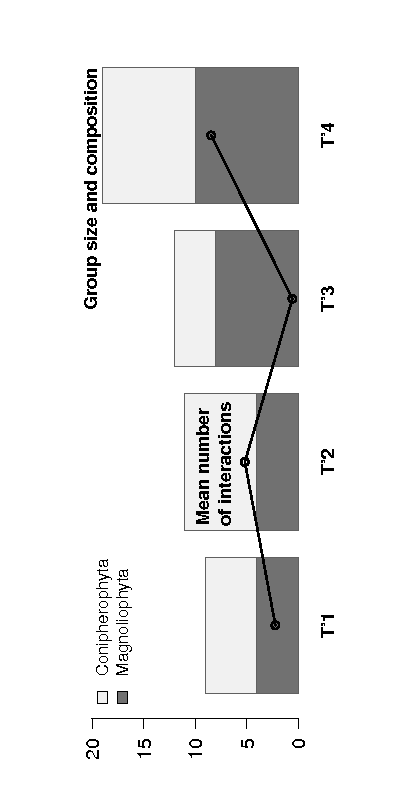
\includegraphics[width=.5\textwidth, trim=150 150 150 150, clip=]{\fignet/MRV10_AoAS_Q4_group}
    \end{tabular}
  \end{tabular}
  }

